\scanpage{4}
\reversemarginpar
\textcircled{\small 20} Vanishing theorem. Cas des espaces homogènes.

\textcircled{\small 21} $H^{*}(X,F)\to H^{\unsure{*|x}}(X_{0},F_{0})$ ($X_{0}$ fermé dans $X$\inserted{\unsure{coh.|ch.} étale}), quand est-ce un isom ? Suffit-il que ce soit vrai en dim $0$ ? Cas $X=\operatorname{Spec} A$, $X_{0}=\unsure{\operatorname{Spe}|\operatorname{Spec}|\operatorname{Sp}} A/\unsure{I|J}$, $A$ $I$-adique séparé complet. Cas de la localisation étale le long de $X_{0}\subset X$, $X$ affine.

22)\margin{travail \unsure{Saavedra} en train}% slanted
\hspace{.4em}Structure des catégorielles abéliennes avec produit tensoriel $\pm$ rigide, en termes de \unsure{représentation|représentations} linéaires des groupes proalgébriques, et de \unsure{représentation|représentations} de gerbes.... \inserted{(préliminaire algébrique à \unsure{le|la} théorie des motifs).}

\figure{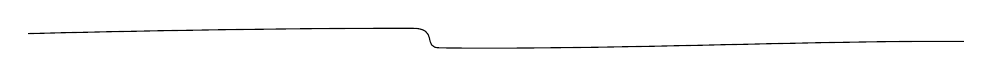
\begin{tikzpicture}[x=.98\linewidth,y=1ex]\draw (0,0) .. controls (.18,.35) and (.32,.45) .. (.41,.45) .. controls (.44,.45) and (.42,-1.2) .. (.44,-1.2) .. controls (.63,-1.35) and (.83,-.6) .. (1,-.65);\end{tikzpicture}}
\par\noindent\uline{Pour \unsure{memoire|mémoire}}

\diagram{\resizebox{\linewidth}{!}{\begin{tikzcd}[ampersand replacement=\&,column sep=2.2em,row sep=0pt,cells={nodes={inner sep=0pt}}]
{\left.\begin{array}{@{}l@{}}
\otimes\ \text{\unsure{Résolution|Résoluton} des singularités.}\\[.8ex]
\otimes\ \text{Pureté cohomologique.}\\[.8ex]
\text{Changement de base régu}\overset{\text{\scriptsize\unsure{?}}}{\text{li}}\text{er}\\[-.3ex]
\qquad\text{\inserted{en cohomologie.}}
\end{array}\right\}}
\arrow[r,Rightarrow,yshift=1.1em]
\arrow[r,Rightarrow,yshift=-1.2em]
\& {\begin{array}{@{}l@{}}
\text{dualité locale}=\text{bidualité,}\\[-.3ex]
\qquad\text{pour la top étale}\\[.8ex]
\text{\unsure{th|ths} de finitude pour morphisme}\\[-.3ex]
\qquad\text{\inserted{de type fini}}\\[-.3ex]
\text{etc etc}
\end{array}}
\end{tikzcd}}}

Dimension cohomologique des \unsure{morphismes} affines.

$\otimes$ \unsure{Théorème|Théorèmes} de finitude genre Grauert.

$\otimes$ Théories \deleted{\unsure{rig|rigide}} type rigide-analytiques.

Questions dans SGA \unsure{1961|1962}

\figure{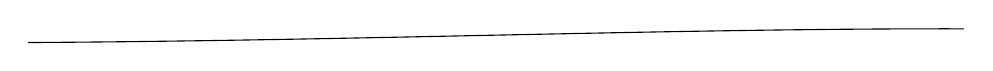
\begin{tikzpicture}[x=.98\linewidth,y=1ex]\draw (0,0) .. controls (.35,.15) and (.7,1.2) .. (1,1.15);\end{tikzpicture}}

\shortstack{23)\\[-.5ex]\scriptsize$\unsure{\times|*}$} Théorie de Chow pour Schémas \deleted{\unsure{qq|qcq} réguliers} ayant un faisceau inversible ample (équivalence rationnelle \unsure{des|de}\unsure{,} cycles). L'image inverse par $f:\unsure{X'|X}\to Y$ doit être définie, sous seule condition que $Y$ soit régulier.

\tikz[baseline=(num.base)]{\node[draw,circle,inner sep=.7pt] (num) {\shortstack{24\\[-.5ex]\scriptsize$\times$}};}
\margin{Réponse négative Griffiths pour question 1\textsuperscript{o}}% slanted
\hspace{.4em}Sur une variété projective lisse connexe de dim $3$ sur $k$ corps \unsure{algébriqmt|algébriquemt|algébriquement} \unsure{clos|clés}, un $1$-cycle num. équiv. à $0$ est-il $\unsure{\tau|t}$-équivalent à zéro ? \inserted{En dim $4$, cycle de dim $2$ équiv. num $=$ équiv. hom ??\unsure{,|'}}
% archive sheet number: 3
\normalmarginpar

